\section{Large numbers of areas}
\label{sec:bayarea}

\setlength{\parindent}{0pt}

\subsection{Data augmentation}
\label{sec:data_aug}

For small rate matrices, transition probabilities of beginning in state $i$ and ending in state $j$ equal the matrix exponential of the underlying rate matrix, scaled by the elapsed time of the process.
This integrates over all unobserved transition events during the time interval $t$.
Unfortunately, computing the matrix exponential scales poorly as the state space increases, i.e. $O(n^4)$ for $n$ states.

Alternatively, the probability of beginning in state $i$ and ending in state $j$ can be computed easily when the explicit series of event types and times are known.
While we will never know the exact history of events, we can use stochastic mapping in conjunction with Markov chain Monte Carlo (MCMC) to repeatedly sample range evolution histories that are consistent with the ranges observed in the study taxa at the tips of the phylogeny.
This technique is called data augmentation. It was first applied in phylogenetics to tertiary structure-dependent evolution of protein-coding nucleotide sequences \citep{robinson03}, and later extended to range evolution in \citet{landis13}.

Using data augmentation, we will approximate {Prob$\left( \textbf{X}_{aug}, \theta \mid \textbf{X}_{obs}, T, M \right)$}, where $\textbf{X}_{obs}$ is the range data observed at the tips, $\textbf{X}_{aug}$ is the distribution of ancestral range reconstructions over the phylogeny, $T$, where $\textbf{X}_{aug}$ is inferred jointly with the parameters, $\theta$, assuming the range evolution model, $M$, that describes $\textbf{Q}$ above.
From a Bayesian perspective, $\textbf{X}_{aug}$ is effectively treated as part of the parameter space in the posterior distribution.
Just as MCMC evaluates the posterior distribution for sampled parameter values, the same is done for sampled character histories.
Thus, ancestral range reconstructions are a by-product of data augmentation, which are often of primary interest to biogeographers.

You may wonder why matrix exponentiation works fine for molecular substitution models and large multiple sequence alignments.
It is the non-independence of character evolution that induces large state spaces, along with cladogenic processes that affect the entire set of characters (e.g. non-identical range inheritance following speciation).
Molecular substitution models typically assume each character in an alignment evolves independently, which may be justified by the ability of recombination to degrade linkage disequilibrium over geological time scales.
Conveniently, this keeps \textbf{Q} small even for datasets with many sites.

\subsection{Large rate matrices and distance-dependent dispersal}
\label{sec:rate_map}

A rate matrix may be represented compactly as the rate function
\[
q^{(a)}_{\textbf{y},\textbf{z}} =
\begin{cases}
\lambda_0 & \text{if $z_a=0$} \\
\lambda_1 & \text{if $z_a=1$} \\
0 & \text{\textbf{y} and \textbf{z} differ in more than one area}
\end{cases}.
\]

where $\textbf{y}$ and $\textbf{z}$ are the ``from'' and ``to'' ranges and $a$ is the area that changes, $\lambda_0$ is the per-area rate of loss, and $\lambda_1$ is the per-area rate of gain.
For example, $q^{(1)}_{011,111}$ is the rate of range expansion for $011 \rightarrow 111$ to gain area $1$, which equals $\lambda_1$.
Note the rate of more than one event occurring simultaneously is zero, so a range must expand twice by one area in order to expand by two areas.
This model is analogous to the Jukes-Cantor model for three independent characters with binary states, except the all-zero ``null range'' is forbidden.

Extending this idea, we may reasonably expect that a range expansion event into an area depends on which nearby areas are currently inhabited, which imposes non-independence between characters.
The transition rate might then appear as
\[
q^{(a)}_{\textbf{y},\textbf{z}} =
\begin{cases}
\lambda_0 & \text{if $z_a=0$}  \\
\lambda_1 \eta(\textbf{y}, \textbf{z}, a, \beta) & \text{if $z_a=1$} \\
0 & \mathbf{y} = 00...0 \\
0 & \text{\textbf{y} and \textbf{z} differ in more than one area}
\end{cases}.
\]

For this tutorial, you can take $\eta(\cdot)$ to adjust the rate of range expansion into area $a$ by considering how close it is to the current range, $\textbf{y}$ relative to the closeness of all other areas unoccupied by the taxon.
The $\beta$ parameter rescales the importance of geographic distance between two areas by a power law.
Importantly, $\eta(\cdot) = 1$ when $\beta=0$, meaning geographic distance between areas is irrelevant.
Moreover, when $\beta > 0$, $\eta(\cdot) < 1$ when area $a$ is relatively distant and $\eta(\cdot) > 1$ when area $a$ is relatively close.
See \citet{landis13} for a full description of the model.

{\bf \framebox{?}} Write down a rate function where the per-area rates of gain and loss depend on the number of currently occupied areas.

\subsection{Specifying a data augmented DEC model}

As previously, start by setting your working directory,

\begin{snugshade}
\begin{lstlisting}
setwd("/Users/arwallace/projects/RB_Biogeography_tutorial/")
\end{lstlisting}
\end{snugshade}

then create helper variables for file handling,

\begin{snugshade}
\begin{lstlisting}
fp      = "./"
area_fn = fp + "data/earth25.still.atlas.txt"
data_fn = fp + "data/primates_bg_n25.nex"
tree_fn = fp + "data/primates.tree"
out_str = "bg_3"
\end{lstlisting}
\end{snugshade}

read in our tree,

\begin{snugshade}
\begin{lstlisting}
tree  <- readTrees(in_fp + data_fn)[1]
\end{lstlisting}
\end{snugshade}

populate our range observations,

\begin{snugshade}
\begin{lstlisting}
data    = readDiscreteCharacterData(in_fp + data_fn)
\end{lstlisting}
\end{snugshade}

and read in our geographical information (for details, see Section XX).

\begin{snugshade}
\begin{lstlisting}
atlas   = readAtlas(in_fp + area_fn)
n_areas = atlas.nAreas()
\end{lstlisting}
\end{snugshade}

Lastly, create index variables to populate our move and monitor vectors,

\begin{snugshade}
\begin{lstlisting}
mvi = 1
mni = 1
\end{lstlisting}
\end{snugshade}

and assign the number of generations to run the MCMC analysis

\begin{snugshade}
\begin{lstlisting}
ngen = 500000
\end{lstlisting}
\end{snugshade}

To later interpret ancestral state monitors phylogenetically, save a copy of {\tt tree} annotated with internal node indexes.

\begin{snugshade}
\begin{lstlisting}
write(tree,filename=tree_fn+".index.tre")
\end{lstlisting}
\end{snugshade}

Proceeding with the model configuration, we'll first create our rate matrix that determines the rate of per-area gain and loss given the current geographical layout of the range.
In RevBayes, data-augmented CTMC analyses require {\tt RateMap} functions to determine event rates, which differ from the familiar {\tt RateMatrix} functions that include {\tt fnJC} and {\tt fnGTR} as members.
In their simplest form, {\tt RateMap} functions generate the rates of change over the full set of characters, where each character evolves according to a provided {\tt RateMatrix} function.
Additionally, a {\tt RateMap} accepts a rate modifier function that induces some correlation structure to character change evolution.
In this section, we'll be creating a biogeographic {\tt RateMap} function for the dispersal-extinction process given in Section \ref{sec:rate_map}.

First, create a biogeographical clock to scale the rate of range evolution.

\begin{snugshade}
\begin{lstlisting}
clock_bg ~ dnExp(10)
moves[mvi++] = mvScale(clock_bg, lambda=0.5, weight=5.0)
\end{lstlisting}
\end{snugshade}

Next, instantiate a simplex of gain and loss rates, distributed by a flat Dirichlet prior,

\begin{snugshade}
\begin{lstlisting}
glr ~ dnDirichlet([1,1])
moves[mvi++] = mvSimplexElementScale(glr, alpha=30.0, weight=5.0)
\end{lstlisting}
\end{snugshade}

and use deterministic nodes to assign the rates nicknames.

\begin{snugshade}
\begin{lstlisting}
r_gain := glr[1]
r_loss := glr[2]
\end{lstlisting}
\end{snugshade}

Insert the simplex into the rate matrix {\tt $q_area$}, which gives the average rate of area gain and loss per area.

\begin{snugshade}
\begin{lstlisting}
q_area := fnFreeBinary(glr)
\end{lstlisting}
\end{snugshade}

Next, we will create {\tt dp} to represent the $\beta$ parameter, which determines the importance of geographical distance to dispersal.
Remember that values of $\beta$ far from zero means distance is important.
So, if we we assign a prior that pulls $\beta$ towards zero, then posterior values of $\beta$ far from zero indicate the range data are informative of the importance of distance to dispersal.
We'll use an exponential distribution with mean 1.0 as a prior for {\tt dp}.

\begin{snugshade}
\begin{lstlisting}
dp ~ dnExponential(10.0)
moves[mvi++] = mvScale(x=dp, lambda=0.5, tune=true, weight=5.0)
\end{lstlisting}
\end{snugshade}

We will also create a deterministic node to modify the rate of dispersal between areas by evaluating {\tt dp} and {\tt atlas}.
This node is determined by the function {\tt fnBiogeoGRM}, where GRM stands for ``geographical rate modifier'', and plays the role of the $\eta(\cdot)$ rate-modifier function mentioned earlier.
We will tell the {\tt fnBiogeoGRM} function to modify dispersal rates based on distances and whether or not the area exists during an epoch.

\begin{snugshade}
\begin{lstlisting}
grm := fnBiogeoGRM(atlas=atlas, distancePower=dp, useDistance=true)
\end{lstlisting}
\end{snugshade}

Now we need a deterministic node to represent the rate matrix, {\bf Q}.
To determine the value of this node, we'll use the function {\tt fnBiogeoDE} to assign our model parameters to transition rates as described in the introduction.
As input, we'll pass our gain and loss rates, {\tt q\_area}, our geographical rate modifier, {\tt grm}, and the biogeographical clock {\tt clock\_bg}.
In addition, we'll inform the function of the number of areas in our analysis and whether we will allow species to be absent in all areas (i.e. have the null range).

\begin{snugshade}
\begin{lstlisting}
q_range := fnBiogeoDE(gainLossRates=q_area, branchRates=clock_bg, geoRateMod=grm, numAreas=n_areas, forbidExtinction=true)
\end{lstlisting}
\end{snugshade}

As with the simple DEC model, we assign a flat Dirichlet prior over cladogenic event type probabilities

\begin{snugshade}
\begin{lstlisting}
clado_prob ~ dnDirichlet( [1, 1, 1] )
widespread_sympatry := clado_prob[1]
subset_sympatry     := clado_prob[2]
allopatry           := clado_prob[3]
moves[mvi++] = mvSimplexElementScale(clado_prob, alpha=20.0, weight=5.0)
\end{lstlisting}
\end{snugshade}

Finally, the data evolve according to a phylogenetic CTMC process. Here, we decalre a stochastic node using {\tt dnPhyloDACTMC} where {\tt DA} indicates the distribution requires data augmentation to compute the likelihood rather than Felsenstein's pruning algorithm.
To create the distribution, we must pass it our {\tt tree} and {\tt q\_range} objects, but additionally inform the distribution that it will be using a biogeographic model, that it will introduce the simple cladogenic range evolution events described in \citet{ree08} ({\tt useCladogenesis=true}), and that it will assign zero probability to a transition away from the null range state.

\begin{snugshade}
\begin{lstlisting}
m ~ dnPhyloDACTMC(tree=tree, Q=q_range, cladoProbs=clado_prob, type="Biogeo", forbidExtinction=true, useCladogenesis=true)
\end{lstlisting}
\end{snugshade}


So we may evaluate the graphical model's likelihood, we tell the CTMC to observe the {\tt data} object, which then primes the model with data-augmented character histories.

Now {\tt m} has a defined likelihood value.
\begin{snugshade}
\begin{lstlisting}
m.clamp(data)
m.lnProbability()
   -156.0288
\end{lstlisting}
\end{snugshade}

To integrate over the space of possible range histories, we still need to add moves to propose new data augmented histories.
The major challenge to sampling character histories is ensuring the character histories are consistent with the observations at the tips of the tree.
The proposals in this tutorial use \citet{nielsen02}'s rejection sampling algorithm, with some modifications to account for cladogenic events and epoch-based rate maps.

The basic idea is simple.
Each time a character history proposal is called, it selects a node at random from the tree.
Branch history proposals propose a new character history to a single randomly-chosen branch.
Node history proposals propose a new character history for the three branches connecting to a randomly chosen node, in addition to the cladogenic state of the node itself.

For each proposal, each character's history is resampled with probability {\tt lambda} -- i.e. {\tt lambda=0.01} resamples 1\% of characters, while {\tt lambda=1.} resamples all characters.
Once the new character history is proposed, the likelihood of the model is evaluated and the MCMC accepts or rejects the new state according to e.g. the Metropolis-Hastings algorithm.

Cladogenic events require special considerations during sampling, so we indicate {\tt type="Biogeo"}.
Currently, only rejection-sampling is available for cladogenic histories, hence {\tt proposal="rejection"}. Finally, we apply high {\tt weight} values to the proposals since the larger the state space is, the more character history proposals needed to effectively integrate over the space of sample paths.

Let's create the character history moves as follows: conservative character history updates for paths and nodes, with {\tt lambda=0.05}

\begin{snugshade}
\begin{lstlisting}
moves[mvi++] = mvCharacterHistory(ctmc=m, qmap=q_range, tree=tree, lambda=0.05, type="Biogeo", graph="node", proposal="rejection", weight=100.0)
moves[mvi++] = mvCharacterHistory(ctmc=m, qmap=q_range, tree=tree, lambda=0.05, type="Biogeo", graph="branch", proposal="rejection", weight=100.0)
\end{lstlisting}
\end{snugshade}

and the same proposals for more radical character history updates, with {\tt lambda=1.0}

\begin{snugshade}
\begin{lstlisting}
moves[mvi++] = mvCharacterHistory(ctmc=m, qmap=q_range, tree=tree, lambda=1.0, type="Biogeo", graph="node", proposal="rejection", weight=40.0)
moves[mvi++] = mvCharacterHistory(ctmc=m, qmap=q_range, tree=tree, lambda=1.0, type="Biogeo", graph="branch", proposal="rejection", weight=40.0)
\end{lstlisting}
\end{snugshade}

Next, create the model object,

\begin{snugshade}
\begin{lstlisting}
my_model = model(m)
\end{lstlisting}
\end{snugshade}

and monitors for our simple parameters.

\begin{snugshade}
\begin{lstlisting}
monitors[mni++] = mnScreen(clock_bg, r_gain, r_loss, dp, subset_sympatry, allopatry, widespread_sympatry, printgen=100)
monitors[mni++] = mnFile(clock_bg, r_gain, r_loss, dp, subset_sympatry, allopatry, widespread_sympatry, filename=out_fn+".params.txt", printgen=10)
\end{lstlisting}
\end{snugshade}

Like any parameter, we can sample the augmented range histories from the MCMC to approximate the posterior distribution of range histories.
This is statistically equivalent to generating ancestral state reconstructions from a posterior distribution via stochastic mapping.
We will extract these reconstructions using special monitors designed for the {\tt dnPhyloDACTMC} distribution.

Next, we will create {\tt mnCharHistoryNewick} monitors to record the sampled character history states for each node in the tree.
This monitor has two {\tt style} options: {\tt counts} reports the number of gains and losses per branch in a tab-delimited Tracer-readable format;  {\tt events} reports richer information of what happens along a branch, anagenically and cladogenically, using an extended Newick format.
How to read these file formats will be discussed in more detail in Section \ref{sec:bg_out}.

\begin{snugshade}
\begin{lstlisting}
monitors[mni++] = mnCharHistoryNewick(filename=out_fn+".events.txt", ctmc=m, tree=tree, printgen=100, style="events")
monitors[mni++] = mnCharHistoryNewick(filename=out_fn+".counts.txt", ctmc=m, tree=tree, printgen=100, style="counts")

\end{lstlisting}
\end{snugshade}

As our last monitor,{\tt mnCharHistoryNhx} records character history values throughout the MCMC analysis, then stores some simple posterior summary statistics as a Nexus file.
These summary statistics could be computed from the previously mentioned monitor output files, but {\tt mnCharHistoryNhx} provides a simple way to produce Phylowood-compatible files.
We will also discuss this file's format in more detail later in the tutorial.

\begin{snugshade}
\begin{lstlisting}
monitors[mni++] = mnCharHistoryNhx(filename=out_fn+".phw.txt", ctmc=m, tree=tree, atlas=atlas, samplegen=100, maxgen=ngen, burnin=0.5)
\end{lstlisting}
\end{snugshade}

Finally, create the MCMC object

\begin{snugshade}
\begin{lstlisting}
my_mcmc = mcmc(my_model, monitors, moves)
\end{lstlisting}
\end{snugshade}

and run

\begin{snugshade}
\begin{lstlisting}
my_mcmc.run(generations=ngen)
\end{lstlisting}
\end{snugshade}

The posterior surface over character histories is highly multimodal, so this analysis takes a long time to mix.
If you're following this tutorial in a lab setting, you should proceed using the pre-analysed output files provided in {\tt ./completed\_output}.

\subsection{Analysis output}
\label{sec:bg_out}

You will need a node-indexed phylogeny to interpret ancestral state reconstructions. First, open FigTree and load the Newick tree stored in {\tt data/primates.tree.index.tre}. Expand ``Node Labels'' and change ``Display'' to the custom node label. All sampled characters have a node index, which corresponds to the branch ancestral to the indexed node.

\begin{centering}
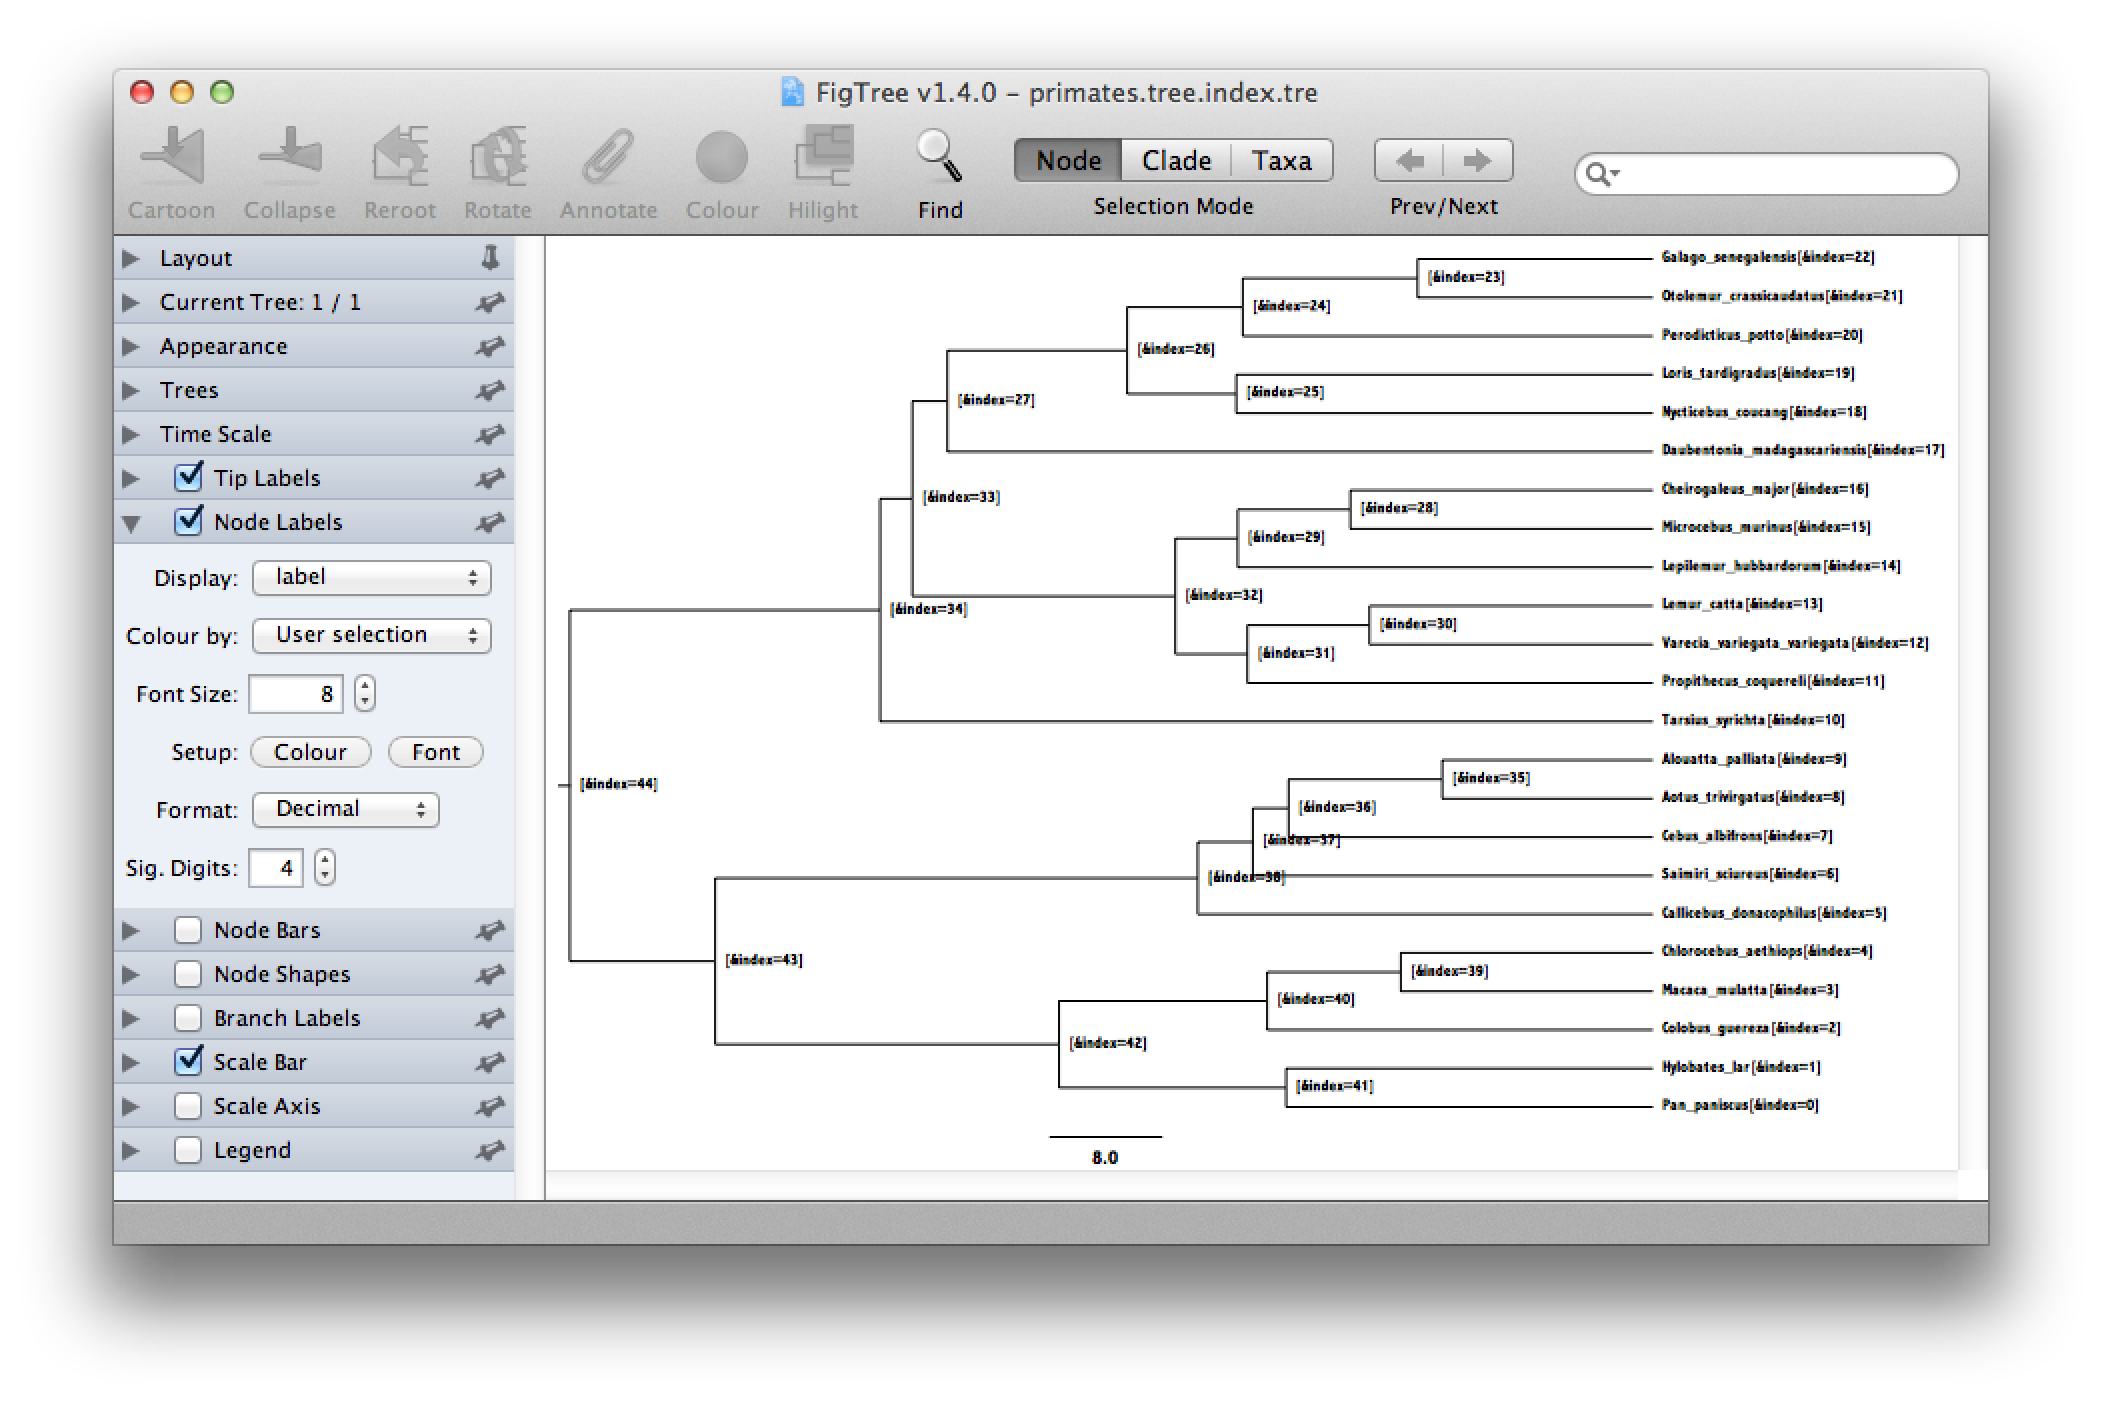
\includegraphics[width=4in]{figures/figtree_node_label}
\end{centering}

We'll focus some attention on node 42, the most recent common ancestor of chimps and macaques, designated as the Old World most recent common ancestor (MRCA).

\subsubsection{Biogeographic event counts from {\tt mnCharHistoryNewick}}

Recording stochastic mappings in a Tracer-compatible format requires some summarization.
This monitor generates a tab-delimited file where the number of events of each type for each branch is recorded.

Open {\tt ./output/bg\_3.counts.txt} in a text editor.

\begin{framed}
\begin{lstlisting}[style=textboxSmall]  % \listingsfont, columns=texcl]
kkkddd
Iter	Posterior	Likelihood	Prior	t_s0	t_s1	t_c0	t_c1	t_c2	t_c3	b0_s0	b0_s1	b0_c	...
0	-6518.54	-6519.25	0.706823	977	839	22	0	0	0	38	28	0	...
10	-583.147	-585.333	2.186240	66	37	3	7	9	3	2	1	2	...
20	-296.540	-297.340	0.799755	20	25	15	1	3	3	0	1	0	...
30	-276.284	-277.257	0.972918	17	24	14	0	4	4	0	1	0	...
40	-266.569	-266.948	0.379624	18	23	15	1	3	3	0	1	3	...
...
\end{lstlisting}
\end{framed}

For example, {\tt b0\_s1} gives the number of areas that are gained for the branch leading to the node indexed 0.
Referencing FigTree, we see this corresponds to chimpanzees.
{\tt b0\_c} gives the cladogenic event type that gives rise to the chimp lineage, where narrow sympatry, widespread sympatry, subset sympatry, and allopatry are recorded as {\tt 0}, {\tt 1}, {\tt 2}, and {\tt 3}, respectively. The columns {\tt t\_s0} and {\tt t\_s1} give the sum of events over all branches. {\tt t\_c0}, {\tt t\_c1}, {\tt t\_c2}, and {\tt t\_c3} give the total number of narrow sympatric, widespread sympatric, subset sympatric, and allopatric cladogenic events over the entire tree.

\subsection{Biogeographic event histories from {\tt mnCharHistoryNewick}}

For more detailed data exploration, this analysis also provides annotated Newick strings with the complete character mappings for the tree.
(This file format is a bit unwieldy and under revision.)

\noindent \\ \impmark Open {\tt ./output/bg\_3.events.txt} in a text editor.

Each iteration records the data-augmented character history (stochastic mapping) using metadata labels, which, for an internal node, looks like

\begin{snugshade}
\begin{lstlisting}
[&index=42;nd=0000000000000101000000000;pa=0000000000000100000000000;ch0=0000000000000101000000000;ch1=0000000000000001000000000;cs=s;bn=41;ev={{t:0.138033,a:39.4458,s:1,i:15}}]
\end{lstlisting}
\end{snugshade}

Having consulted FigTree earlier, we know node 42 is the Old World MRCA.
The branch began with the range {\tt pa=0000000000000100000000000} and terminated in the state {\tt nd=0000000000000101000000000}.
Since this node is not a tip node, it represents a speciation event, so the daughter ranges are also given, {\tt ch0=0000000000000101000000000} and {\tt ch1=0000000000000001000000000}.
The cladogenic state for this speciation event was subset sympatric, {\tt cs=s}, rather than sympatric (wide or narrow; {\tt w} or  {\tt n}) or allopatric ({\tt a}).

Anagenic dispersal and extinction events occurring along the lineage leading to node 42 are recorded in {\tt ev}, where each event has a time (relative to the absolute branch length), absolute age, state (into), and character index ({\tt t}, {\tt a}, {\tt s}, {\tt i}, resp.).
Potentially, {\tt ev} contains multiple events.
For this posterior sample, the MRCA of chimps and macaques dispersed into East Africa 39.4458 million years ago, which is consistent with the ranges recorded by {\tt pa} and {\tt nd}.

Although we have stochastic mappings under the posterior distribution, the remaining challenge is to summarize them into something useful. The Python script {\tt bg\_parse.py} is provided to manipulate this data format. Below are a few examples of interesting features of the posterior.

\noindent \\ \impmark  Open a Python console and read in the events.

\begin{snugshade}
\begin{lstlisting}
> cd RevBayes_scripts
> python

...

>>> from bg_parse import *
>>> d=get_events(fn="../output/bg_3.events.txt")
\end{lstlisting}
\end{snugshade}

By default, {\tt get\_events()} extracts a dictionary-of-dictionaries from the posterior event samples.
A dictionary is very much like a vector, so this can be thought of as similar to a two-dimensional matrix.
The first key corresponds to the node (branch) whose MCMC samples you'd like to retrieve, while the second dictionary's keys are the columns correspond to MCMC states and values specific to that node. For example, say we are interested in the last five cladogenic states sampled for node 42, Old World MRCA,
\begin{snugshade}
\begin{lstlisting}
>>> dd[42].keys()
['ch1', 'iteration', 'bn', 'nd', 'ch0', 'prior', 'posterior', 'pa', 'cs', 'ev', 'likelihood']
>>> dd[42]['cs'][-5:]
['widespread_sympatry', 'widespread_sympatry', 'widespread_sympatry', 'widespread_sympatry', 'widespread_sympatry']
\end{lstlisting}
\end{snugshade}

To get the {\tt n=1} highest-valued sample for a branch by its posterior value
\begin{snugshade}
\begin{lstlisting}
>>> get_best(dd[42],n=1,p='posterior')
{'prior': [-0.524716], 'iteration': [46700], 'bn': [41], 'nd': [[0, 0, 0, 0, 0, 0, 0, 0, 0, 0, 0, 1, 0, 1, 0, 1, 0, 0, 0, 0, 0, 0, 0, 0, 0]], 'ch0': [[0, 0, 0, 0, 0, 0, 0, 0, 0, 0, 0, 1, 0, 1, 0, 1, 0, 0, 0, 0, 0, 0, 0, 0, 0]], 'ch1': [[0, 0, 0, 0, 0, 0, 0, 0, 0, 0, 0, 1, 0, 1, 0, 1, 0, 0, 0, 0, 0, 0, 0, 0, 0]], 'posterior': [-95.7676], 'pa': [[0, 0, 0, 0, 0, 0, 0, 0, 0, 0, 0, 1, 0, 1, 0, 1, 0, 0, 0, 0, 0, 0, 0, 0, 0]], 'cs': ['widespread_sympatry'], 'ev': [[]], 'likelihood': [-95.2429]}
\end{lstlisting}
\end{snugshade}

More data-exploration functions are found in {\tt bg\_parse.py}.

\subsection{Phylowood animation file (\texttt{./output/bg\_3.nhx.txt})}

Because this data is very high-dimensional, we'll use an external data exploration tool to look at range evolution.
This file summarizes the MCMC output from a RevBayes biogeographical analysis as a Nexus-formatted file, which is used by Phylowood to generate interactive animations to explore biogeographic reconstructions.

\noindent \\ \impmark Open \texttt{http://mlandis.github.io/phylowood}.

\noindent \\ \impmark Drag and drop \texttt{./output/bg\_3.nhx.txt} into the text field.

\begin{figure}[H]
\centering
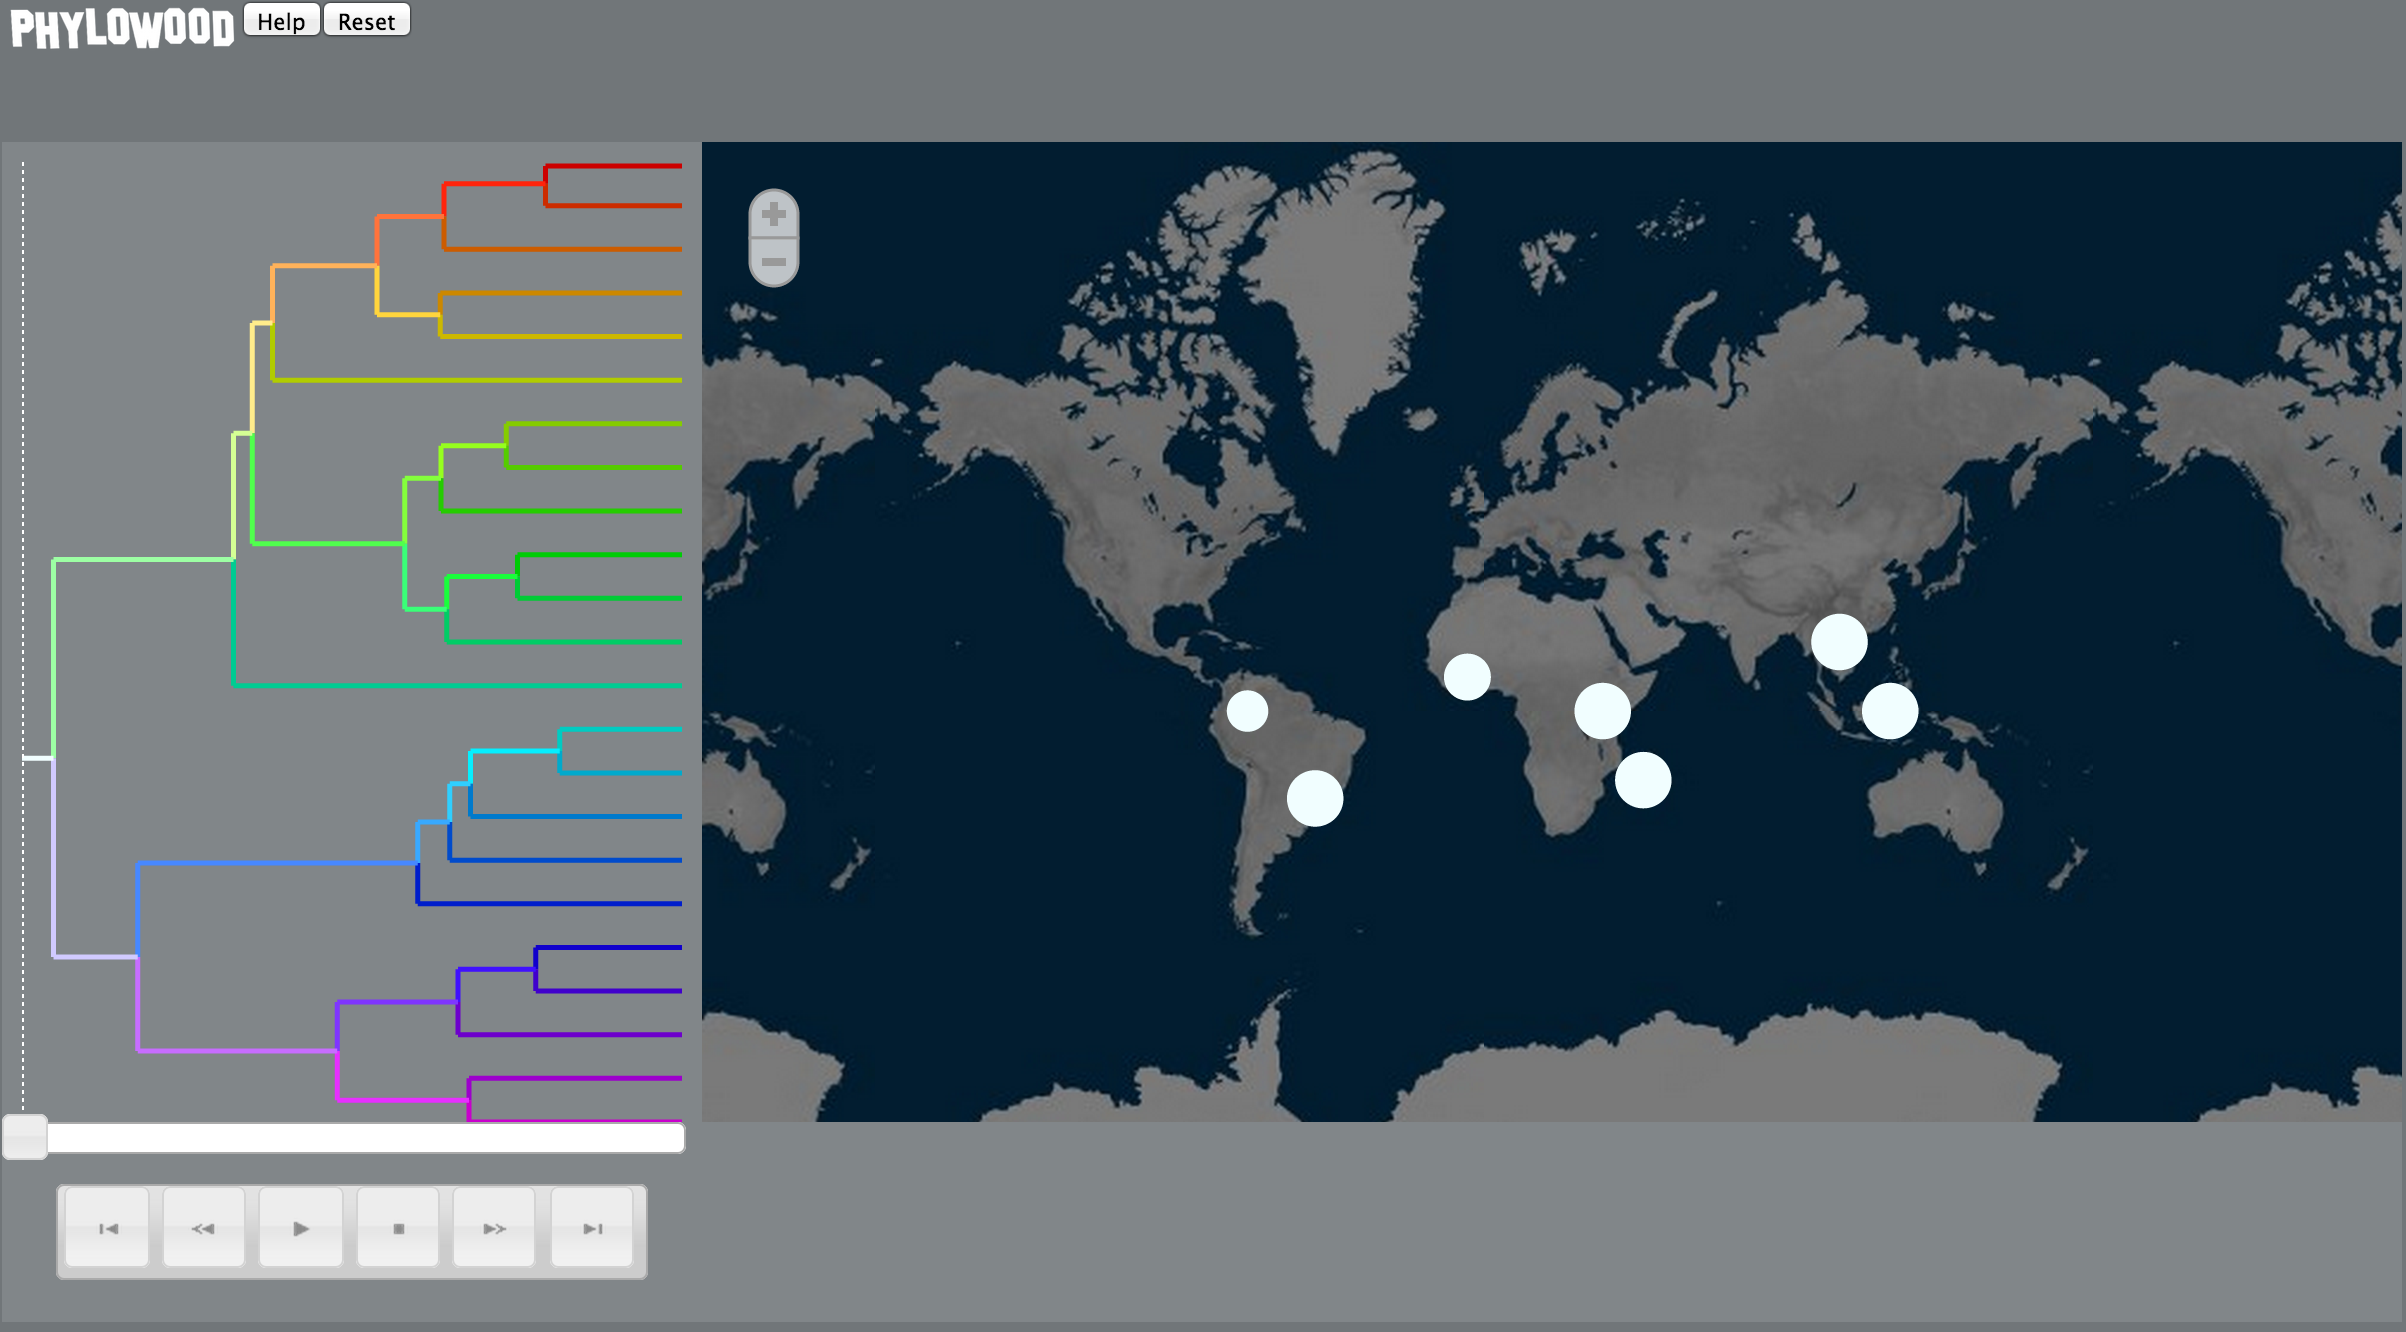
\includegraphics[width=4in]{figures/phw_mrca}
\caption{Phylowood frame showing posterior ancestral range of root node.}
\end{figure}

\noindent \\ \impmark Click the Play button to view the animation. \\

Notice the primate MRCA range is very widespread with six areas. This is

There are three control panels to help you filter data: the media panel, the map panel, and the phylogeny panel.
The media buttons correspond to Beginning, Slow/Rewind, Play, Stop, Fast Forward, Ending (from left to right).
The animation will play the timeframe corresponding to the slider.

\noindent \\ \impmark Drag the slider to the right (the present).

\begin{figure}[H]
\centering
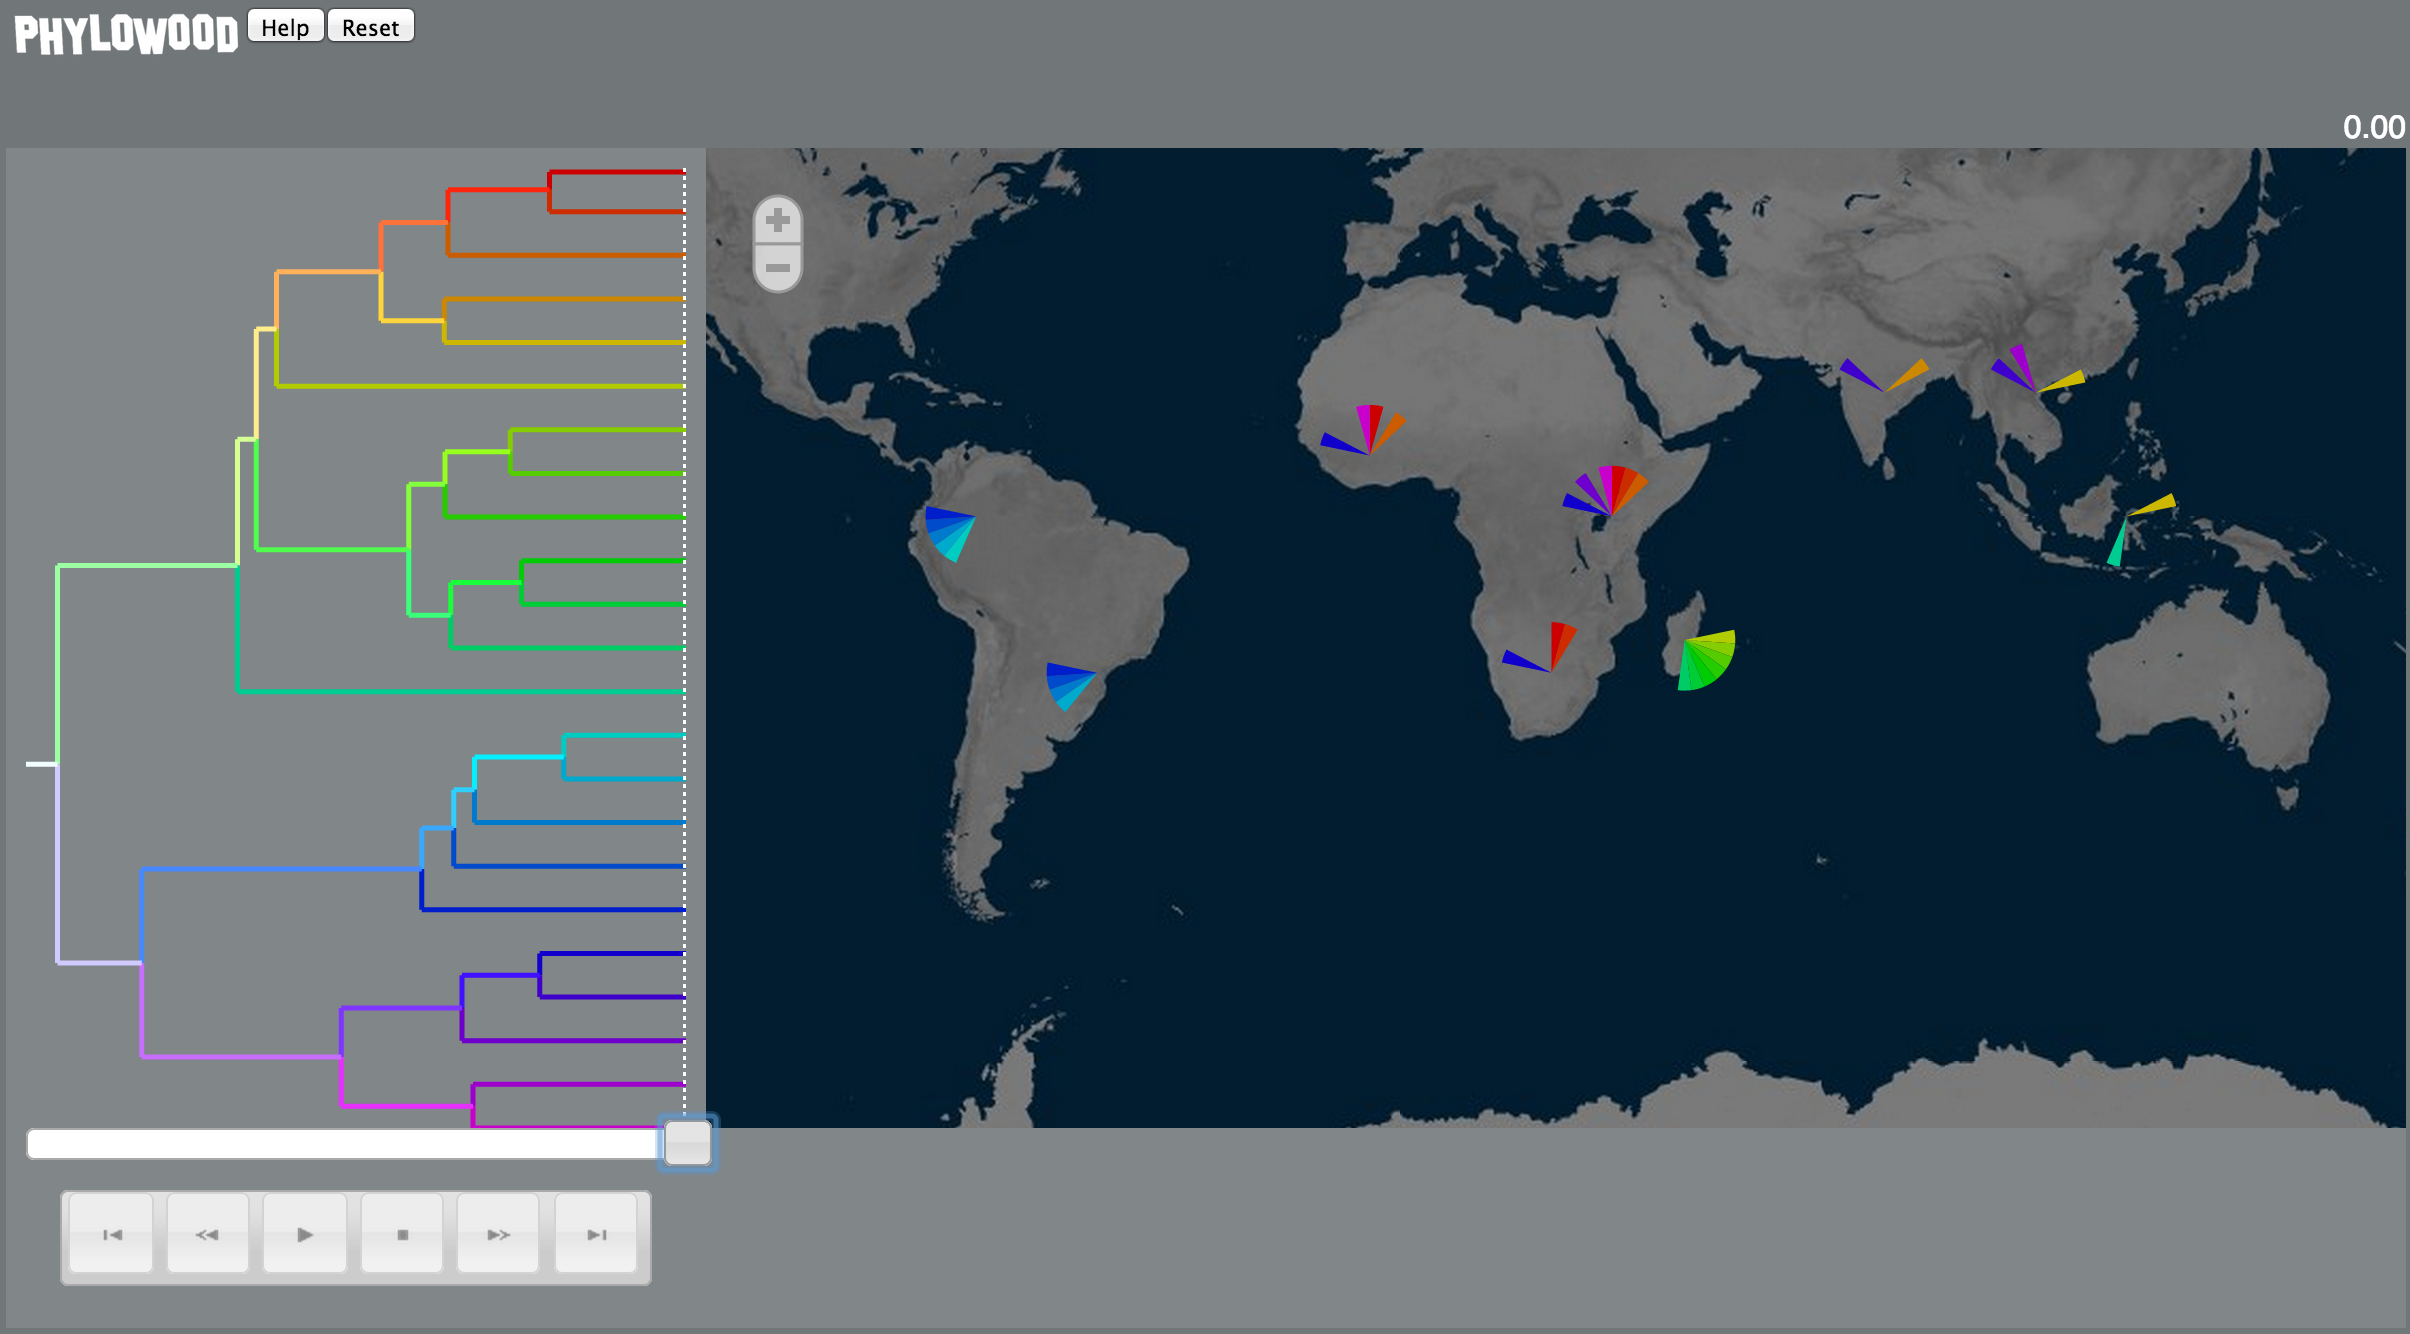
\includegraphics[width=4in]{figures/phw_all}
\caption{Phylowood frame showing distribution of extant taxon ranges.}
\end{figure}

\noindent \\ \impmark Pan and zoom around the map.\\

Marker colors correspond to the phylogenetic lineages in the phylogeny panel.
Markers are split into slices and (loosely) sorted phylogenetically, so nearby slices are generally closely related.
At divergence events, a marker's radius is proportional to the marginal posterior probability the node was present in the area at that time.
Between divergence events, marker's radius is simply an interpolation of the values at the two endpoints.
Some information about geological constraints and cladogenic events is lost.

\noindent \\ \impmark Mouseover an area to learn which lineage it belongs to and its presence probability. \\

Since it's difficult to see how specific clades evolve with so many taxa, Phylowood offers two ways to filter taxa from the animation.
We call the set of a lineage, all its ancestral lineages towards the root, and all descendant lineages a phylogenetic heritage.
The root's heritage is the entire clade.
A leaf node's heritage is a path from the tip to the root.

\noindent \\ \impmark Mouseover a lineage to temporarily highlight the lineage's heritage. Remove the mouseover to remove the highlight effect. \\

The highlight effect is temporary and quickly allows you to single out lineages of interest during animation.
Phylowood also offers a masking effect that persists until an unmask command is issued.

\noindent \\ \impmark Double-click the white root branch to mask the root node's heritage (all lineages). Single click a lineage to unmask that lineage's heritage. \\

\begin{figure}[H]
\centering
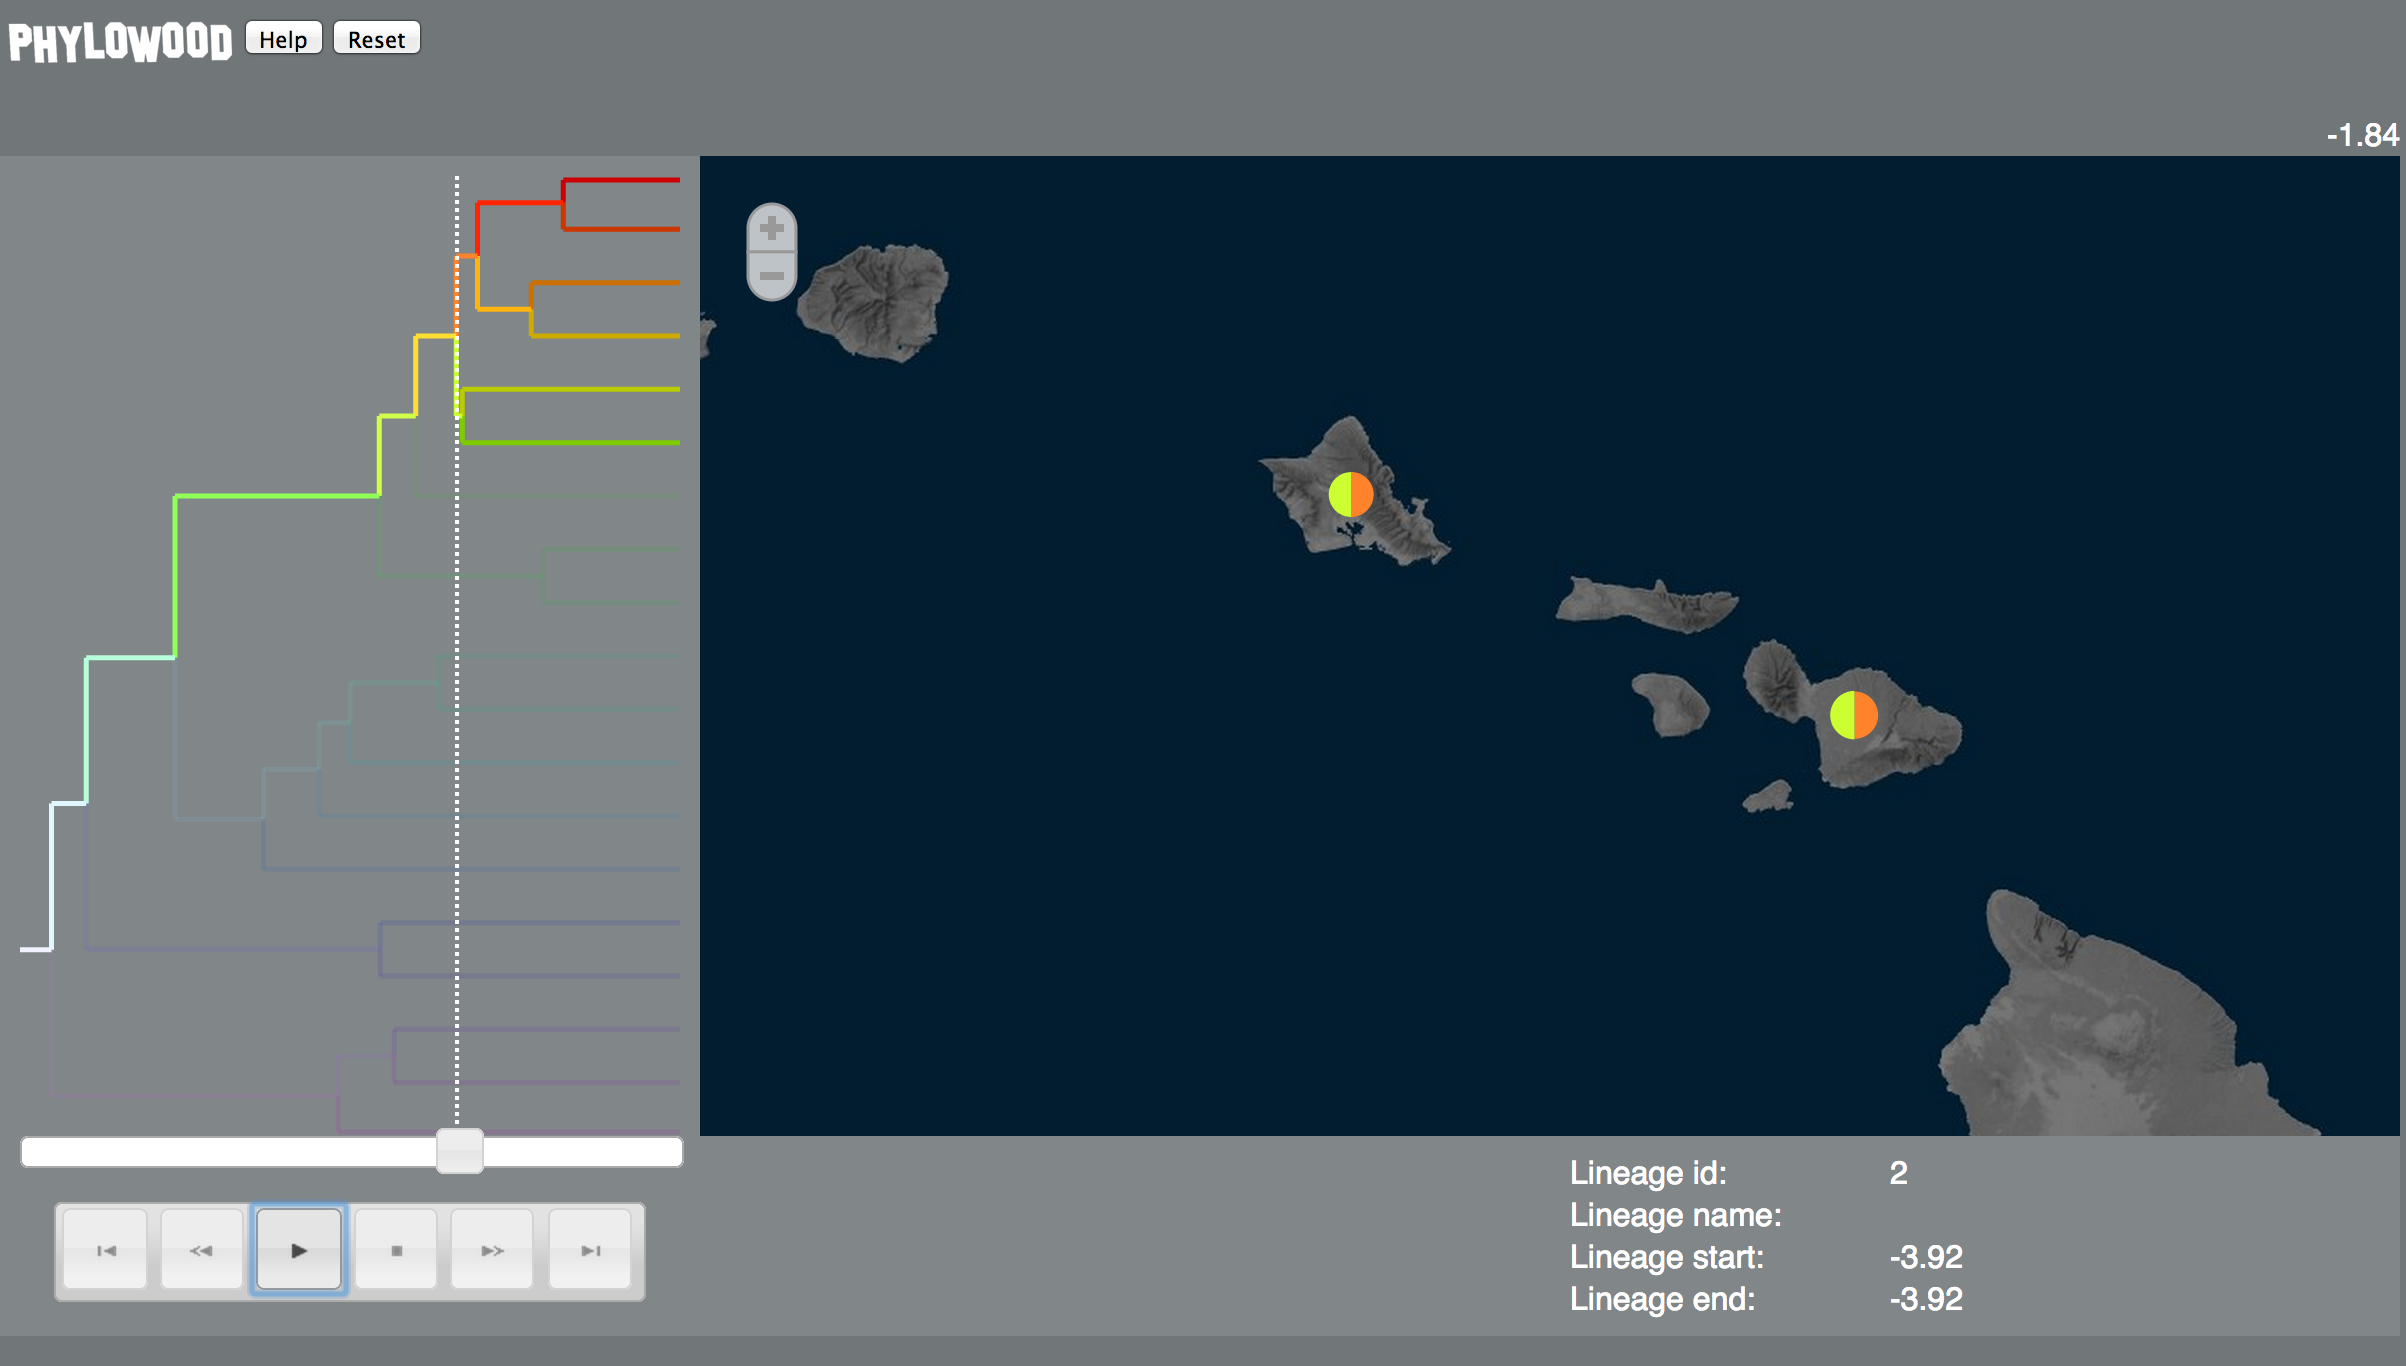
\includegraphics[width=4in]{figures/phw_br23}
\caption{Phylowood frame highlighting the posterior range for Old World MRCA.}
\end{figure}

Now that the masking effects are in place, you're free to interact with other map components.
In addition, the area of marker sizes is only distributed among unmasked lineages.

Visit \texttt{https://github.com/mlandis/phylowood/wiki} to learn more about Phylowood.

\subsection{Exercises}

\begin{itemize}
\item (Under construction.)
\end{itemize}
